\documentclass[a4paper,14pt]{extarticle}

% Путь до папки с общими шаблонами
\newcommand{\pathToCommonFolder}{/home/denilai/Documents/repos/latex/Common}
% Название работы в титуле
\newcommand{\workname}{Отчет по практической работе №7}
% Название дисциплины в титуле
\newcommand{\discipline}{Разработка и программирование микропроцессорных систем}
% Название кафедры в титуле
\newcommand{\kafedra}{Кафедра вычислительной техники}
% Тема работы в титуле
\newcommand{\theme}{Изучение системы команд микроконтроллера семейства MCS-51}
% Должность преподавателя в титуле
\newcommand{\rang}{ассистент кафедры ВТ}
% ФИО преподавателя в титуле
\newcommand{\teacherfio}{Р.~Э.~Семенов}
\newcommand{\studentfio}{К.~Ю.~Денисов}
\newcommand{\signature}{\pathToCommonFolder/denisov-signature}
\newcommand{\heading}[1]{\multicolumn{1}{c}{#1}}

%\usepackage[tableposition=top,singlelinecheck=false]{caption}
%\captionsetup*[lstlisting]{font={small, it}}

% установка размера шрифта для всего документа
%\fontsize{20pt}{18pt}\selectfont


% Вставка заготовки преамбулы
% Этот шаблон документа разработан в 2014 году
% Данилом Фёдоровых (danil@fedorovykh.ru) 
% для использования в курсе 
% <<Документы и презентации в \LaTeX>>, записанном НИУ ВШЭ
% для Coursera.org: http://coursera.org/course/latex .
% Исходная версия шаблона --- 
% https://www.writelatex.com/coursera/latex/5.3

% В этом документе преамбула

% Для корректного использования русских символов в формулах
% пакеты hyperref и настройки, связанные с ним, стоит загуржать
% перед загрузкой пакета mathtext



% поддержка русских букв
% кодировка шрифта
%\usepackage[T2A]{fontenc} 
\usepackage{pscyr}

% использование ненумеровонного абзаца с добавлением его в содержаниеl

\newcommand{\anonsection}[1]{\section*{#1}\addcontentsline{toc}{section}{#1}}
\newcommand{\sectionunderl}[1]{\section*{\underline{#1}}}


% настройка окружения enumerate
\usepackage{enumitem}
\setlist{noitemsep}
\setlist[enumerate]{labelsep=*, leftmargin=1.5pc}

\usepackage{hyperref}

% сначала ставить \usepackage{extsizes} % Возможность сделать 14-й шрифт
% для корректной установки полей вставлять преамбулу следует в последнюю очередь (но перед дерективой замены \rmdefault)
\usepackage[top=20mm,bottom=25mm,left=35mm,right=20mm]{geometry} % Простой способ задавать поля

\hypersetup{				% Гиперссылки
	unicode=true,           % русские буквы в раздела PDF
	pdftitle={Заголовок},   % Заголовок
	pdfauthor={Автор},      % Автор
	pdfsubject={Тема},      % Тема
	pdfcreator={Создатель}, % Создатель
	pdfproducer={Производитель}, % Производитель
	pdfkeywords={keyword1} {key2} {key3}, % Ключевые слова
	colorlinks=true,       	% false: ссылки в рамках; true: цветные ссылки
	linkcolor=red,          % внутренние ссылки
	citecolor=black,        % на библиографию
	filecolor=magenta,      % на файлы
	urlcolor=blue           % на URL
}

%%% Работа с русским языком
\usepackage{cmap}					% поиск в PDF
\usepackage{mathtext} 				% русские буквы в формулах
\usepackage[T2A]{fontenc}			% кодировка
\usepackage[utf8]{inputenc}			% кодировка исходного текста
\usepackage[english,russian]{babel}	% локализация и переносы
\usepackage{indentfirst}
\frenchspacing

%для изменения названия списка иллюстраций
\usepackage{tocloft}


\renewcommand{\epsilon}{\ensuremath{\varepsilon}}
\renewcommand{\phi}{\ensuremath{\varphi}}
\renewcommand{\kappa}{\ensuremath{\varkappa}}
\renewcommand{\le}{\ensuremath{\leqslant}}
\renewcommand{\leq}{\ensuremath{\leqslant}}
\renewcommand{\ge}{\ensuremath{\geqslant}}
\renewcommand{\geq}{\ensuremath{\geqslant}}
\renewcommand{\emptyset}{\varnothing}

% Изменения параметров списка иллюстраций
\renewcommand{\cftfigfont}{Рисунок } % добавляем везде "Рисунок" перед номером
\addto\captionsrussian{\renewcommand\listfigurename{Список иллюстративного материала}}

\newcommand{\tm}{\texttrademark\ }
\newcommand{\reg}{\textregistered\ }


%%% Дополнительная работа с математикой
\usepackage{amsmath,amsfonts,amssymb,amsthm,mathtools} % AMS
\usepackage{icomma} % "Умная" запятая: $0,2$ --- число, $0, 2$ --- перечисление

%% Номера формул
%\mathtoolsset{showonlyrefs=true} % Показывать номера только у тех формул, на которые есть \eqref{} в тексте.
%\usepackage{leqno} % Нумереация формул слева

%% Свои команды
\DeclareMathOperator{\sgn}{\mathop{sgn}}

%% Перенос знаков в формулах (по Львовскому)
\newcommand*{\hm}[1]{#1\nobreak\discretionary{}
{\hbox{$\mathsurround=0pt #1$}}{}}


% отступ для первого абзаца главы или параграфа
%\usepackage{indentfirst}

%%% Работа с картинками
\usepackage{graphicx}  % Для вставки рисунков
\graphicspath{{images/}{screnshots/}}  % папки с картинками
\DeclareGraphicsExtensions{.pdf,.png,.jpg}
\setlength\fboxsep{3pt} % Отступ рамки \fbox{} от рисунка
\setlength\fboxrule{1pt} % Толщина линий рамки \fbox{}
\usepackage{wrapfig} % Обтекание рисунков текстом

%%% Работа с таблицами
\usepackage{array,tabularx,tabulary,booktabs} % Дополнительная работа с таблицами
\usepackage{longtable}  % Длинные таблицы
\usepackage{multirow} % Слияние строк в таблице

%%% Теоремы
\theoremstyle{plain} % Это стиль по умолчанию, его можно не переопределять.
\newtheorem{theorem}{Теорема}[section]
\newtheorem{proposition}[theorem]{Утверждение}

\theoremstyle{plain} % Это стиль по умолчанию, его можно не переопределять.
\newtheorem{work}{Практическая работа}[part]


 
 
\theoremstyle{definition} % "Определение"
\newtheorem{corollary}{Следствие}[theorem]
\newtheorem{problem}{Задача}[section]
 
\theoremstyle{remark} % "Примечание"
\newtheorem*{nonum}{Решение}



%%% Программирование
\usepackage{etoolbox} % логические операторы

%%% Страница

%	\usepackage{fancyhdr} % Колонтитулы
% 	\pagestyle{fancy}
%   \renewcommand{\headrulewidth}{0pt}  % Толщина линейки, отчеркивающей верхний колонтитул
% 	\lfoot{Нижний левый}
% 	\rfoot{Нижний правый}
% 	\rhead{Верхний правый}
% 	\chead{Верхний в центре}
% 	\lhead{Верхний левый}
%	\cfoot{Нижний в центре} % По умолчанию здесь номер страницы

\usepackage{setspace} % Интерлиньяж
\onehalfspacing % Интерлиньяж 1.5
%\doublespacing % Интерлиньяж 2
%\singlespacing % Интерлиньяж 1

\usepackage{lastpage} % Узнать, сколько всего страниц в документе.

\usepackage{soul} % Модификаторы начертания


\usepackage[usenames,dvipsnames,svgnames,table,rgb]{xcolor}


\usepackage{csquotes} % Еще инструменты для ссылок

%\usepackage[style=authoryear,maxcitenames=2,backend=biber,sorting=nty]{biblatex}

\usepackage{multicol} % Несколько колонок

\usepackage{tikz} % Работа с графикой
\usepackage{pgfplots}
\usepackage{pgfplotstable}

% модуль для вставки рыбы
\usepackage{blindtext}

\usepackage{listings}
\usepackage{color}


% для поворота отдельной страницы. Использовать окружение \landscape
\usepackage{pdflscape} 
\usepackage{rotating} 


\definecolor{mygreen}{rgb}{0,0.6,0}
\definecolor{mygray}{rgb}{0.5,0.5,0.5}
\definecolor{mymauve}{rgb}{0.58,0,0.82}


% пример импорта файла
%\lstinputlisting{/home/denilai/repomy/conf/distributions}

\lstset{
	language=Python,
	basicstyle=\footnotesize,        % the size of the fonts that are used for the code
	numbers=left,                    % where to put the line-numbers; possible values are (none, left, right)
	numbersep=5pt,                   % how far the line-numbers are from the code
	numberstyle=\tiny\color{mygray}, % the style that is used for the line-numbers
	stepnumber=2,                    % the step between two line-numbers. If it's 1, each line will be numbered
	% Tab - 2 пробела
	tabsize=2,    
	% Автоматический перенос строк
	breaklines=true,
	frame=single,
	breakatwhitespace=true,
	title=\lstname 
}



\author{Денисов Кирилл ИВБО-02-19}
\title{Практическая работа №7}
\date{\today}

\setcounter{withouttheme}{1}

% установка полуторного интервала
% \usepackage{setspace}  
% \onehalfspacing

% использовать Times New Roman
\renewcommand{\rmdefault}{ftm}
\begin{document}
	\maketitle
	
\begin{enumerate}
	\item Включим пересылку IPv4 трафика на виртуальной машине под управлением Astra Linux, дописав ее в конец файла /etc/sysctl.conf с помощью команды 
	
	\begin{lstlisting}
	# echo "net.ipv4.ip\_forward=1" >> /etc/sysctl.conf \end{lstlisting}
	
	Результат приведен на рисунке \ref{fig:---2022-03-30-16-54-58}.
% TODO: \usepackage{graphicx} required
\begin{figure}[h!]
	\centering
	\includegraphics[width=0.5\linewidth]{"images/Снимок экрана от 2022-03-30 16-54-58"}
	\caption{}
	\label{fig:---2022-03-30-16-54-58}
\end{figure}
	
	Применим изменения с помощью команды
	
	\begin{lstlisting}
	# sysctl -p \end{lstlisting}
	
	Результат приведен на рисунке \ref{fig:---2022-03-30-16-56-42}.
	
% TODO: \usepackage{graphicx} required
\begin{figure}[h!]
	\centering
	\includegraphics[width=0.5\linewidth]{"images/Снимок экрана от 2022-03-30 16-56-42"}
	\caption{}
	\label{fig:---2022-03-30-16-56-42}
\end{figure}

	\item Для включения маскарадинга на выходном интерфейсе eth1 следует выполнить команду 
	
	\begin{lstlisting}
	# iptables -t nat -A POSTROUTING -o eth0 -j MASQUERADE\end{lstlisting}
	
	\item Включим файервол ufw с помощью команды 
	
	\begin{lstlisting}
	# ufw enable\end{lstlisting}
	
	Проверим работу файервола ufw выполнив команду
		\begin{lstlisting}
		# ufw status\end{lstlisting}

	\item Теперь необходимо разрешить транзитные соединения командой 
	
	\begin{lstlisting}
	# ufw default allow routed\end{lstlisting}
	
	Результат приведен на рисунке \ref{fig:---2022-03-30-17-15-09}.
	
	% TODO: \usepackage{graphicx} required
	\begin{figure}[h!]
		\centering
		\includegraphics[width=0.5\linewidth]{"images/Снимок экрана от 2022-03-30 17-15-09"}
		\caption{}
		\label{fig:---2022-03-30-17-15-09}
	\end{figure}
	\newpage
	\item Дополним файл /etc/ufw/before.rules следующим правилом.
	
	
	
	\begin{lstlisting}[caption=/etc/ufw/before.rules, label=sdfsdf]
		*nat
		:POSTROUTING ACCEPT [0:0]
		#Forwardtraffic from eth1 through eth0.
		-A POSTROUTING -s 192.168.1.0/24 -o eth0 -j MASQUERADE
		COMMIT	\end{lstlisting}
	
	\item После этого перезагрузим ufw командами 
	\begin{lstlisting}
	# ufw disable
	# ufw enable\end{lstlisting}
	
	\item Проверим наличие нашего правила командой
	
	\begin{lstlisting}
	# iptables -t nat -L
	# iptables-save \end{lstlisting}
	
	Результат приведен на рисунке \ref{fig:---2022-03-30-17-15-28}.
	
% TODO: \usepackage{graphicx} required
\begin{figure}[h!]
	\centering
	\includegraphics[width=0.5\linewidth]{"images/Снимок экрана от 2022-03-30 17-15-28"}
	\caption{}
	\label{fig:---2022-03-30-17-15-28}
\end{figure}
	
	\item Произведем настройку интерфейса eth1, путем внесения изменений в файл /etc/network/intefaces.
	
	\item Перезапустим службу networking командой
	
	\begin{lstlisting}
	# systemctl restart networking\end{lstlisting}
	
	
	Результат приведен на рисунке \ref{fig:---2022-03-30-17-22-22}.
% TODO: \usepackage{graphicx} required
\begin{figure}[h!]
	\centering
	\includegraphics[width=0.5\linewidth]{"images/Снимок экрана от 2022-03-30 17-22-22"}
	\caption{}
	\label{fig:---2022-03-30-17-22-22}
\end{figure}

	\item Установим dhcp сервер с помощью пакетного менеджера 
	\begin{lstlisting}
	# apt install isc-dhcp-server\end{lstlisting}
	
	
	Результат приведен на рисунке \ref{fig:---2022-03-30-17-49-27}.
% TODO: \usepackage{graphicx} required
\begin{figure}[h!]
	\centering
	\includegraphics[width=0.5\linewidth]{"images/Снимок экрана от 2022-03-30 17-49-27"}
	\caption{}
	\label{fig:---2022-03-30-17-49-27}
\end{figure}

	Настроим его, отредактировав файл /etc/dhcp/dhcpd.conf 	
	
	
	\begin{lstlisting}[caption=/etc/dhcp/dhcpd.conf, label=sdfsdf]
	subnet 192.168.1.0 netmask 255.255.255.0 {
	range 192.168.1.50 192.168.1.240;
	option routers 192.168.1.1;
	option broadcast-address 192.168.1.255;
	option domain-name-servers 192.168.1.1;
	authoritative;
	}\end{lstlisting}
	
	\item Запустим dhcpd командой
	\begin{lstlisting}
	# systemctl enable --now isc-dhcp-server\end{lstlisting}
	
	
	После перезапуска сервер удачно сконфигурирован. На изображение попали результаты предыдущих перезапусков сервиса.
	
	
	Результат приведен на рисунке \ref{fig:2022-03-3017-44-04}.
% TODO: \usepackage{graphicx} required
\begin{figure}[h!]
	\centering
	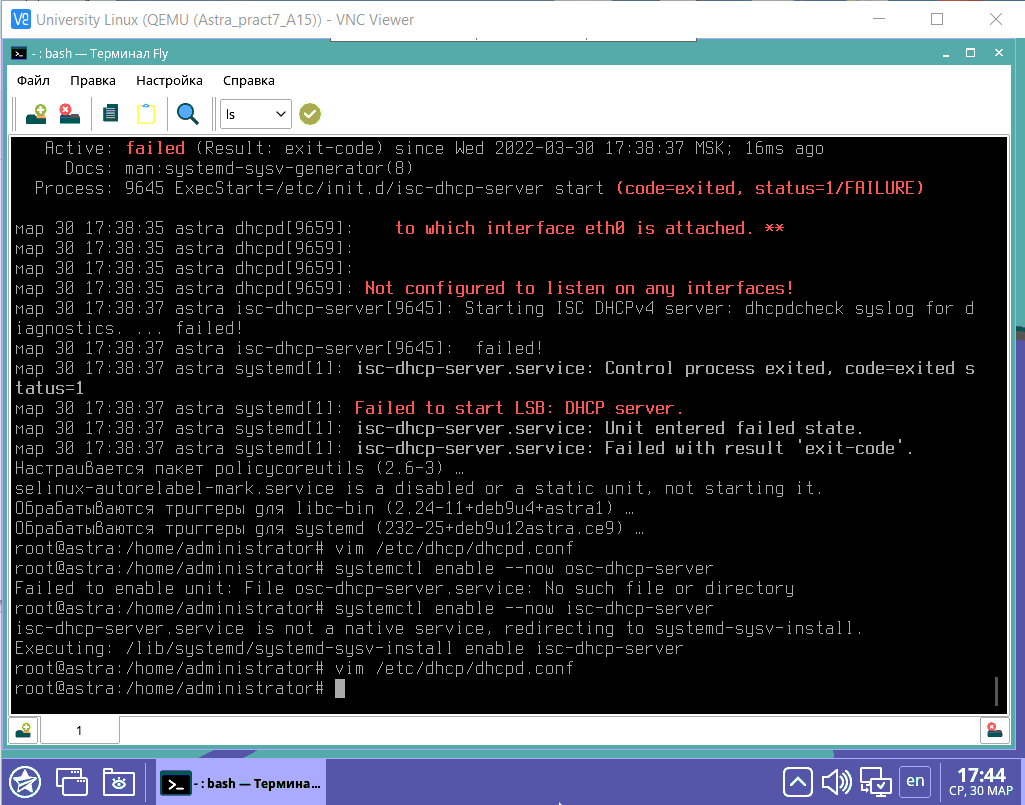
\includegraphics[width=0.5\linewidth]{images/Lesha/2022-03-30_17-44-04}
	\caption{}
	\label{fig:2022-03-3017-44-04}
\end{figure}
\newpage

	\item После этого узел с ОС Windows автоматически получит сетевой адрес из
	заданного диапазона. Проверим работоспособность сети, выполнив в ОС Windows команду
	ping –n 10 8.8.8.8
	
	
	Результат приведен на рисунке \ref{fig:2022-03-3018-01-20}.
% TODO: \usepackage{graphicx} required
\begin{figure}[h!]
	\centering
	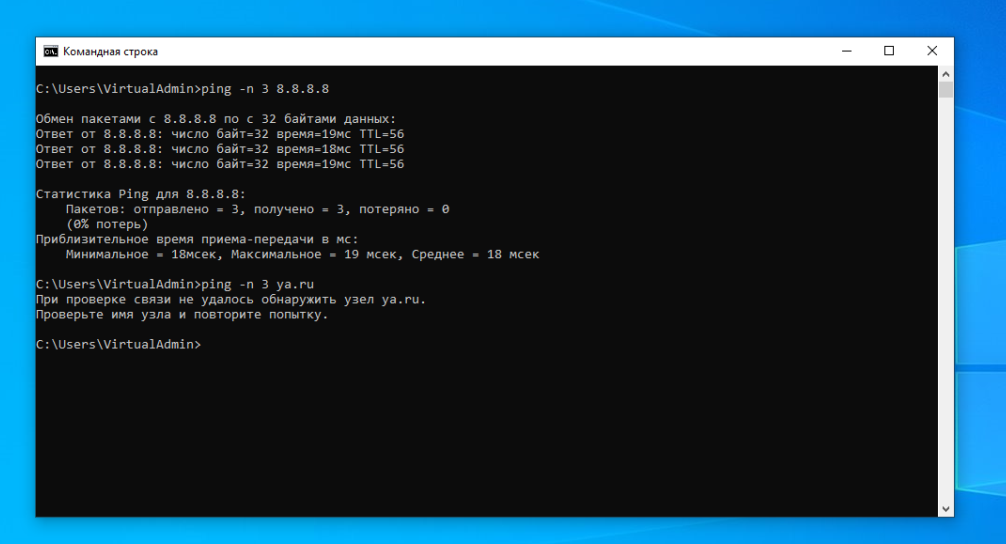
\includegraphics[width=0.7\linewidth]{images/Lesha/2022-03-30_18-01-20}
	\caption{}
	\label{fig:2022-03-3018-01-20}
\end{figure}

	\item Установим ISC BIND командой
	
	\begin{lstlisting}
	# apt install bind9\end{lstlisting}
	
	
	\item Запустим службу bind9 с помощью команды	
	\begin{lstlisting}
	# systemctl enable --now bind9\end{lstlisting}
	
	\item Для работы сетевых сервисов необходимо разрешить
	их порты (или профили) в файерволе, для ufw это делается командой
	\begin{lstlisting}
	# ufw allow Bind9\end{lstlisting}
	
	
		Результат приведен на рисунке \ref{fig:2022-03-3018-02-41}.
% TODO: \usepackage{graphicx} required
\begin{figure}[h!]
	\centering
	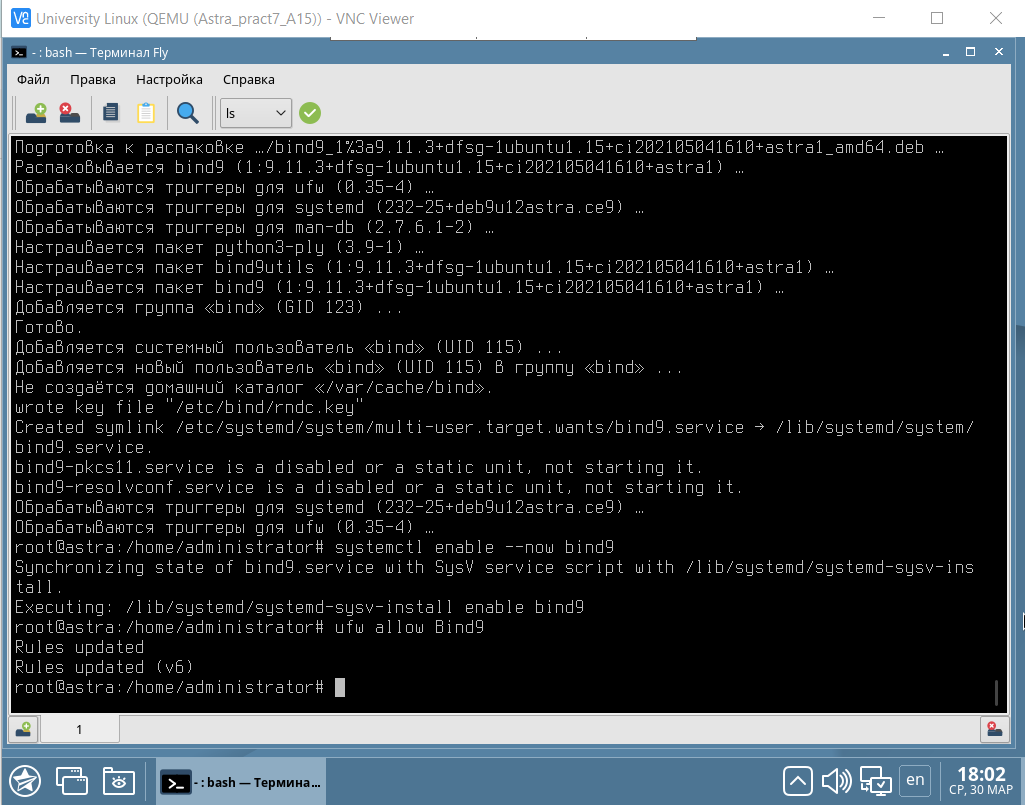
\includegraphics[width=0.5\linewidth]{images/Lesha/2022-03-30_18-02-41}
	\caption{}
	\label{fig:2022-03-3018-02-41}
\end{figure}

После произведения всех перечисленных действия на ВМ с ОС Windows появился доступ в
глобальную сеть без какой-либо дополнительной настройки.

	Результат приведен на рисунке \ref{fig:2022-03-3018-04-09}.
% TODO: \usepackage{graphicx} required
\begin{figure}[h!]
	\centering
	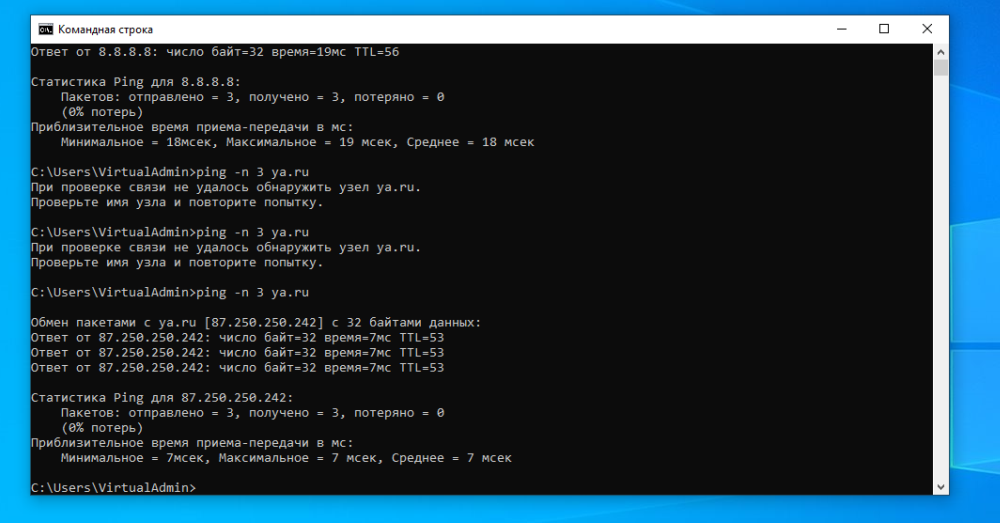
\includegraphics[width=0.7\linewidth]{images/Lesha/2022-03-30_18-04-09}
	\caption{}
	\label{fig:2022-03-3018-04-09}
\end{figure}
	
	
	
\end{enumerate}
\end{document}}